\documentclass[../main.tex]{subfiles}
\begin{document}
\setchapterstyle{kao}
\setchapterpreamble[u]{\margintoc}
\setchapterimage[6.5cm]{Images/intro.jpg}
\chapter[Introduction to the Standard Model]{Introduction to the Standard Model\footnotemark[0]}
\labch{IntroSM}
\section{Particles and Fundamental Interactions}
The Standard Model (SM) is the theory for all fundamental interactions except gravity. How can we organize all the particles we observed so far? Is there an order? Obviously, the answer is yes. We can divide them between particles which mediate forces and particles which are affected by such forces but are not mediators or between elementary and non-elementary particles, stable and unstable and so on.
\[
\begin{aligned}
&\text{Stable particle}&&\text{Reason}\\
\hline
&\gamma && \text{massless}\\
&\text{lightest}\;\nu &&\text{lightest fermion}\\
&e^- &&\text{lightest EM charged particle}\\
&p &&\text{lightest baryon}\\
\hline
\end{aligned}
\]
The photon is massless so it cannot decay into anything. Nowadays we think that neutrinos have a small mass, so the lightest one will be stable. Electron decay would violate U(1)$_{\text{EM}}$, it cannot decay into something that it is neutral so it has to be stable. The stability of the proton is due to the invariance of the Standard Model under baryon number transformations and the modern viewpoint is that this is an accidental symmetry of the Standard Model.\marginnote{We are not going to discuss accidental symmetries here.}\\
All the other particles instead can decay and we can learn something about them by looking at their lifetime because this tells us what kind of interactions they experience.
\renewcommand*{\arraystretch}{1.2}
\begin{center}
    \begin{tabular}{c}
  $\kern-\nulldelimiterspace\left.
  \begin{tabular}{@{}p{0.25\textwidth}p{0.25\textwidth}p{0.25\textwidth}@{}}
    Decay & Lifetime $\tau$ & $c\tau$\\
    \hline
    $n\to pe^-\Bar{\nu}_e$ & 886\,s &$2.7\cdot10^8$\,km \\
    $\mu^-\to e^-\nu_\mu\Bar{\nu}_e$ & $2.2\cdot10^{-6}$\,s & 659\,m\\
    $\pi^-\to \mu^-\nu\Bar{\nu}_\mu$ & $2.6\cdot10^{-8}$\,s & 7.8\,m\\
    $K_L\to\pi l\Bar{\nu}_e$ & $5\cdot10^{-8}$\,s & 15\,m\\
    $\tau\to l^-\Bar{\nu}_e\nu_\tau$ & $0.3\cdot10^{-12}$\,s & 87\,$\mu$m 
  \end{tabular}\right\}$ {Electroweak interaction{\color{white}etic}}
\\
  $\kern-\nulldelimiterspace\left.
  \begin{tabular}{@{}p{0.25\textwidth}p{0.25\textwidth}p{0.25\textwidth}@{}}
  $\pi^0\to\gamma\gamma$ & $8.4\cdot10^{-12}$\,s & 25\,mm\\
  \hline\hline
  \end{tabular}\right\}$ Electromagnetic interaction
\\
$\kern-\nulldelimiterspace\left.
  \begin{tabular}{@{}p{0.25\textwidth}p{0.25\textwidth}p{0.25\textwidth}@{}}
  Resonance & Lifetime $\tau$ & $\Gamma/m$\\
  \hline
  $\rho\to\pi\pi$ & $4.4\cdot10^{-24}$\,s & 0.2\\
  $\Delta\to\pi\pi$ & $5.5\cdot10^{-24}$\,s & 0.1\\
  \end{tabular}\right\}$ {Strong interaction{\color{white}omagneti}}
\end{tabular}
\end{center}
Why are we interested in this list? Well, we see that some decays have a relatively long lifetime, typically of order of 10$^{-6}$-10$^{-8}$ but as it is possible to see it can go up to some hundreds of seconds. This indicates us that they are mediated by \textbf{electroweak interaction}. The $\tau$ is also affected by electroweak interaction despite its shorter lifetime due to some suppressions in its three-body decay. Then there is a sort of gap, particles like $\pi^0$ have a smaller lifetime and they decay through \textbf{electromagnetic interaction}. Resonances are particles which decay so fast that can be only seen as exchange of energy. These decays are mediated by the \textbf{strong force}.\\
Just by looking at lifetimes we were able to identify the fundamental interactions described by the Standard Model:
\begin{itemize}
    \item \underline{Electromagnetism:} long range, $V(r)\sim\frac{1}{r}$
    \item \underline{Weak force:} ($\beta$ decay) short range, $V(r)\sim \frac{e^{-mr}}{r}$ for $m\sim100$\,GeV
    \item \underline{Strong force:} binds the nucleons to form the nuclei, short range because it is confined, $V(r)\sim r$ for $r\lesssim1$\,fm
\end{itemize}
Particles can be classified based on which force they experience. Moreover, we divide the particles in:
\begin{itemize}
    \item \underline{Leptons:} (weak and electromagnetic force) $e,\mu\tay,\nu_e,\nu_\mu,\nu_\tau$
    \item \underline{Hadrons:} (weak, electromagnetic and strong force) $\pi,p,n,k,\dots$
\end{itemize}
\section{Standard Model as an Effective Gauge Theory}
The Standard Model is based upon a gauge paradigm: the fundamental forces are mathematically described by gauge theories. How can we have all these manifestations described by a single representation? The Lagrangian is the same but in different phases: the \textbf{Coulomb phase} for the electromagnetic force, the \textbf{Higgs phase} for the weak force and the \textbf{confinement phase} for the strong force. What is the gauge group associated? 
\[
\text{G}=\text{SU}(3)_{\text{C}}\times\text{SU}(2)_{\text{EW}}\times\text{U}(1)_{\text{Y}}
\]
SU$(3)_{\text{C}}$ gives us 8 gluons, from SU$(2)_{\text{EW}}\times$U$(1)_{\text{Y}}$ we get $W_\mu^\pm, Z_\mu, \gamma$: these are the \textbf{gauge fields} of the SM, in this way we can explain these three forces. It is a renormalizable theory, symmetry breaking happens via a scalar field containing the Higgs boson. SM is an EFT, at high energies the coupling grows and there will be a Landau pole around $10^{24}$\,GeV.\\
For each representation of the field we have three copies, called \textbf{families}.
\begin{table}[h]
        \centering
        \begin{tabular}{c|c|c|c|c}
        Field & SU$(3)_C$ & SU$(2)_{EW}$ & U$(1)_Y$ & SO(3,1) \\
        \hline
        $q_L^i=\begin{pmatrix}u_L\^i\d_L^i
        \end{pmatrix}$ & $\Box$ & $\Box$ & +1/6 & (2,1) \\
        $u_R^i$ & $\Box$ & 1 & +2/3 & (1,2) \\
        $d_R^i$ & $\Box$ & 1 & -1/3 & (1,2) \\
        \hline
        $l_L^i=\begin{pmatrix}\nu_L^i\\e_L^i\end{pmatrix}$ & 1 & $\Box$ & -1/2 & (2,1) \\
        $l_R^i$ & 1 & 1 & -1 & (1,2) \\
        \hline
        $G_\mu^{a=1,\dots,8}$ & Adj & 1 & 0 & (2,2)\\
        $W_\mu^{i=1,2,3}$ & 1 & Adj & 0 & (2,2)\\
        $B_\mu$ & 1 & 1 & 0 & (2,2)\\
        \hline
        $H$ & 1 & $\Box$ & +1/2 & (1,)\\
        \hline
        \end{tabular}
        \caption*{}
        \label{tab:my_label}
    \end{table}
The Standard Model is a chiral theory, left- and right-handed transform in different ways: we cannot write a mass term. There is no right-handed neutrino because we do not need it now, we want the minimum number of fields which reproduce what is observed in nature. At this point, we have to write the Lagrangian:
\[
\pazocal{L}=\pazocal{L}_{kin}+\pazocal{L}_{Yuk}+\pazocal{L}_\theta-V(H)+\text{higher dimension operators}
\]
where the pieces composing the Lagrangian are:
\[
\left\{
\begin{aligned}
&\pazocal{L}_{kin}=-\frac{1}{4}(G_{\mu\nu}^a)^2-\frac{1}{4}(W_{\mu\nu}^i)^2-\frac{1}{4}(B_{\mu\nu})^2+|D_\mu H|^2+\sum_{\{\Psi\}}\sum_{j=1}^{3}\Bar{\Psi}_ji\slashed{D}\Psi_j\\
&\pazocal{L}_\theta=\frac{\theta_0}{32\pi^2}G_{\mu\nu}^a\Tilde{G}^{\mu\nu,a}\\
&\pazocal{L}_{Yuk}=-\sum_{i,j=1}^3\left[\bar{q}_L^i(Y_u)^{ij}H^cu_R^j+\bar{q}_L^i(Y_d)^{ij}Hd_r^j+\bar{l}_L^i(Y_l)^{ij}He_R^j+\text{h.c}\right]
\end{aligned}
\right.
\]
$Y_u$, $Y_d$ and $Y_l$ are $3\times3$ matrices in flavour space. We know that $\Box$ of SU(2) is a pseudo-real representation, $H$ is the $\Box$ of SU(2) so it is always possible to form another $\Box$ of SU(2): $H^c:=i\sigma^2H^*$. It transforms as a doublet, we use it to build the Yukawa coupling and we use $H^c$ because it has hypercharge -1/2.\\
We look at the potential V(H):
\[
V(H)=-\mu^2H^\dagger H+\lambda(H^\dagger H)^2
\]
We have to choose the right parametrization for the Higgs field $H$. We have 4 degrees of freedom, so we can put three of them on an exponential and the last one as a multiplicative constant:
\[
H(x)=e^{i\overset{\mathclap{\tikz \node {$\downarrow$} node [above=1ex] {\footnotesize  Nambu-Goldstone bosons};}}{\chi^i(x)}\sigma^i}\left(\begin{array}{c}0\\\frac{\phi(x)}{\sqrt{2}}\end{array}\right)
\]
Substituting this form of $H$ into the expression for the potential $V(H)$, we find out that this is only a function of $\phi(x)$:
\[
V(H)\xrightarrow[]{}V(\phi)=-\frac{\mu^2}{2}\phi^2+\frac{\lambda}{4}\phi^4
\]
\begin{figure}[h!]
    \centering
    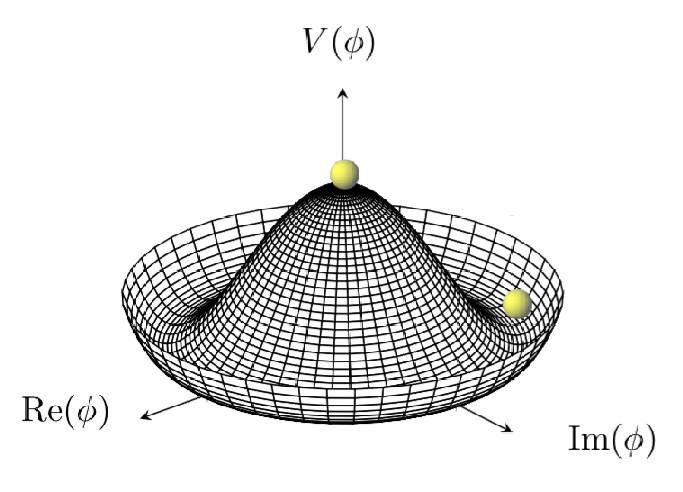
\includegraphics{Images/sombrero.png}
    \caption{Higgs potential has the shape of a Mexican hat ("\textit{sombrero potential}").}
    \labfig{sombrero}
\end{figure}\\
This potential has two minima in $\pm v$, where $v=\sqrt{\mu^2/\lambda}=\langle\phi\rangle$: the field $\phi(x)$ can be written as its mean value plus an excitation which turns out to be the Higgs boson:
\[
\phi(x)=\frac{v+h(x)}{\sqrt{2}}
\]
$h(x)$ is the radial excitation while $\chi(x)$ is the angular excitation: the latter costs no energy since $V(\phi)$ does not depend on $\chi$, therefore the NGBs are massless. We have the SSB mechanism here: how do we understand which symmetry we are breaking? We write the vev and see what symmetry is left invariant.
\[
\langle H(x)\rangle=\frac{1}{\sqrt{2}}\begin{pmatrix}
    0\\v
\end{pmatrix}
\]
Now we act with a combination of generators from SU(2)$\times$U(1), $a_0Y+a_i\sigma_i/2$. We want to see when $(a_0Y+a_i\sigma_i/2)\langle H(x)\rangle=0$.
\begin{align*}
\left(a_0Y+a_i\frac{\sigma_i}{2}\right)\langle H(x)\rangle&=\frac{1}{2}\left(\begin{array}{cc}
    a_0+a_3 & a_1-ia_2 \\
    a_1+ia_2 & a_0-a_3
\end{array}\right)\begin{pmatrix}
    0\\1
\end{pmatrix}\\
&=\frac{1}{2}\begin{pmatrix}
    a_1-ia_2\\a_0-a_3
\end{pmatrix}
\begin{pmatrix}
    0\\1
\end{pmatrix}=\begin{pmatrix}
    0\\0
\end{pmatrix}\Rightarrow\left\{\begin{aligned}
    &a_1=a_2=0\\
    &a_0=a_3
\end{aligned}\right.
\end{align*}
The unbroken generator is $Q=Y+T_3$, the Higgs scalar potential breaks SU$(2)_{EW}\times$U$(1)_Y$ into U$(1)_Q$, i.e. 3+1 generators are broken into 1, resulting in 3 massless modes.\\
We now want to see masses and couplings, so we move in the unitary gauge where $\chi^i=0$. In the unitary gauge the potential will depend on $h(x)$, resulting in:
\[
V(H)=\frac{m_h^2}{2}h^2(x)+\lambda vh^3(x)+\frac{\lambda}{4}h^4(x)+\text{const}
\]
with $m_h^2=2\mu^2=2v^2\lambda$. We need the masses for the vector bosons, so we look at the kinetic term
$|D_\mu H|^2=(D_\mu H)^\dagger(D_\mu H)$:
\[
D_\mu H=\frac{1}{\sqrt{2}}\left[\partial_\mu-\frac{i}{2}(gW_\mu^i\sigma^i+g'Y_WB_\mu)\right]\begin{pmatrix}0 \\ v+h(x)\end{pmatrix}
\]
where $g$ is the gauge coupling of SU(2) and $g'$ the gauge coupling of the hypercharge. At first, we define $W_\mu^\pm:=(W_\mu^2\mp iW_\mu^2)/\sqrt{2}$ and $\sigma^\pm:=(\sigma^1\pm i\sigma^2)/\sqrt{2}$, so that we can write:
\begin{align*}
W_\mu^+\sigma^++W_\mu^-\sigma^-&=\frac{1}{2\sqrt{2}}(W_\mu^1-iW_\mu^2)(\sigma^1+i\sigma^2)+\frac{1}{2\sqrt{2}}(W_\mu^1+iW_\mu^2)(\sigma^1-i\sigma^2)\\
&=\frac{1}{2\sqrt{2}}(W_\mu^1\sigma^1+\cancel{iW_\mu^1\sigma^2}-\cancel{iW_\mu^2\sigma^1}+W_\mu^2\sigma^2)\\
&+\frac{1}{2\sqrt{2}}(W_\mu^1\sigma^1-\cancel{iW_\mu^2\sigma^2}+\cancel{iW_\mu^2\sigma^1}+W_\mu^2\sigma^2)\\
&=\frac{1}{\sqrt{2}}(W_\mu^1\sigma^1+W_\mu^2\sigma^2)
\end{align*}
From which it follows that:
\[
W_\mu^1\sigma^1+W_\mu^2\sigma^2+W_\mu^3\sigma^3=\sqrt{2}(W_\mu^+\sigma^++W_\mu^-\sigma^-)+W_\mu^3\sigma^3
\]
$D_\mu H$ now becomes:
\[
D_\mu H=\frac{1}{\sqrt{2}}\begin{pmatrix}0 \\ \partial_\mu h(x)\end{pmatrix}-\frac{i}{2\sqrt{2}}(gW_\mu^3\sigma^3+g'Y_WB_\mu)\begin{pmatrix}0 \\ v+h(x)\end{pmatrix}-\frac{ig}{2}(W_\mu^+\sigma^++W_\mu^-\sigma^-)\begin{pmatrix}0 \\ v+h(x)\end{pmatrix}
\]
When we act with $\sigma^3$, $\sigma^+$ and $\sigma^-$ on $H(x)$ we get:
\[
\left\{
\begin{aligned}
&\sigma^3H(x)=\left(\begin{array}{cc}
    1 & 0 \\
    0 & -1
\end{array}\right)\left(\begin{array}{c}
  0 \\
  v+h(x)
\end{array}\right)=-\left(\begin{array}{c}
  0 \\
  v+h(x)
\end{array}\right) \\
&\sigma^+H(x)=\left(\begin{array}{cc}
    0 & 1 \\
    0 & 0
\end{array}\right)\left(\begin{array}{c}
  0 \\
  v+h(x)
\end{array}\right)=\left(\begin{array}{c}
  v+h(x) \\
  0
\end{array}\right) \\
&\sigma^-H(x)=\left(\begin{array}{cc}
    0 & 0 \\
    1 & 0
\end{array}\right)\left(\begin{array}{c}
  0 \\
  v+h(x)
\end{array}\right)=\left(\begin{array}{c}
  0 \\
  0
\end{array}\right)
\end{aligned}
\right.
\]
Substituting this into the previous expression for $D_\mu H$, one finds:
\[
D_\mu H=\frac{1}{\sqrt{2}}\begin{pmatrix}0 \\ \partial_\mu h(x)\end{pmatrix}+\frac{i}{2\sqrt{2}}(gW_\mu^3-g'Y_WB_\mu)\begin{pmatrix}0 \\ v+h(x)\end{pmatrix}-\frac{ig}{2}W_\mu^+\begin{pmatrix}v+h(x) \\ 0 \end{pmatrix}
\]
With the same strategy, we compute $(D_\mu H)^\dagger$:
\begin{align*}
(D_\mu H)^\dagger&=\begin{pmatrix}0 & v+h(x)\end{pmatrix}\frac{1}{\sqrt{2}}\left[\partial_\mu+\frac{i}{2}(g\sigma^iW_\mu^i+g'Y_WB_\mu)\right]\\
&=\frac{1}{\sqrt{2}}\begin{pmatrix}0 & \partial_\mu h(x)\end{pmatrix}+\frac{i}{2\sqrt{2}}\begin{pmatrix}0 & v+h(x)\end{pmatrix}(g\sigma^3W_\mu^3-g'Y_WB_\mu)\\
&+\frac{ig}{2}\begin{pmatrix}0 & v+h(x)\end{pmatrix}(\sigma^+W_\mu^++\sigma^-W_\mu^-)\marginnote{We act with the $\sigma$ matrices on the row vector: $\sigma^3$ changes its sign as before, $\sigma^+$ gives a zero while $\sigma^-$ flips it.}\\
&=\frac{1}{\sqrt{2}}\begin{pmatrix}0 & \partial_\mu h(x)\end{pmatrix}-\frac{i}{2\sqrt{2}}\begin{pmatrix}0 & v+h(x)\end{pmatrix}(g'Y_WB_\mu-gW_\mu^3)\\
&+\frac{ig}{2}\begin{pmatrix}v+h(x) & 0\end{pmatrix}W_\mu^-
\end{align*}
We can finally write the full form of $|D_\mu H|^2$:
\begin{align*}
|D_\mu H|^2&=(D_\mu H)^\dagger(D_\mu H)\\
&=\frac{1}{2}(\partial_\mu h(x))^2+\frac{(v+h(x))^2}{8}(gW_\mu^3-g'B_\mu)^2+\frac{g^2}{4}(v+h(x))^2W_\mu^+W_\mu^-\\
&=\frac{1}{2}(\partial_\mu h(x))^2+\frac{v^2}{8}(gW_\mu^3-g'B_\mu)^2\left(1+\frac{h(x)}{v}\right)^2+\frac{g^2v^2}{4}W_\mu^+W_\mu^-\left(1+\frac{h(x)}{v}\right)^2
\end{align*}
Moreover, we can define the mass of the $Z$ and the $W$ boson $m_Z$ and $m_W$ as:
\[
\left\{
\begin{aligned}
m_Z^2&=\frac{g^2+g'^2}{4}v^2\\
m_W^2&=\frac{g^2}{4}v^2
\end{aligned}
\right.
\]
To write $m_Z$ explicitly inside $|D_\mu H|^2$, we perform a rotation. Let $A_\mu$ be the massless field and $Z_\mu$ the massive one:
\[
\left(\begin{array}{c}
     A_\mu \\
     Z_\mu
\end{array}\right)=\left(\begin{array}{cc}
    \cos\theta_W & \sin\theta_W \\
    -\sin\theta_W & \cos\theta_W
\end{array}\right)\left(\begin{array}{c}
     B_\mu \\
     W_\mu^3 
\end{array}\right)\Rightarrow Z_\mu=-\sin\underset{\mathclap{\tikz \node {$\uparrow$} node [below=1ex] {\footnotesize  \href{https://en.wikipedia.org/wiki/Steven_Weinberg}{Weinberg} angle};}}{\theta_W}B_\mu+\cos\theta_WW_\mu^3
\]
To write the mass term $m_Z^2$ in the expression of $|D_\mu H|^2$, we have to perform some tricks:
\[
{\color{red}\frac{g^2+g'^2}{g^2+g'^2}}\frac{v^2}{8}(g'B_\mu-gW_\mu^3)^2=\frac{m_Z^2}{2}\left(\frac{g}{\sqrt{g^2+g'^2}}W_\mu^3-\frac{g'}{\sqrt{g^2+g'^2}}B_\mu\right)^2
\]
To obtain the desired result, we express the Weinberg angle $\theta_W$ in terms of the couplings $g_1$ and $g_2$:
\[
\sin\theta_W:=\frac{g'}{\sqrt{g^2+g'^2}} \quad \cos\theta_W:=\frac{g}{\sqrt{g^2+g'^2}}
\]
$|D_\mu H|^2$ now can be written as:
\[
|D_\mu H|^2=\frac{1}{2}(\partial_\mu h(x))^2+\frac{m_Z^2}{2}Z_\mu Z^\mu\left(1+\frac{h(x)}{v}\right)^2+m_W^2W_\mu^+W_\mu^-\left(1+\frac{h(x)}{v}\right)^2
\]
We have the three fields that will acquire mass, the only remaining massless field is the photon. The mixing angle $\theta_W$ also gives the relationship between the masses of the $W$ and the $Z$ boson:
\[
\frac{m_W^2}{m_Z^2}=\frac{g^2}{g^2+g'^2}=\cos^2\theta_W
\]
from which we can define the quantity $\rho$: 
\[
\rho=\frac{m_W^2}{m_Z^2\cos^2\theta_W}
\]
which is equal to 1 at tree level, but this symmetry gets broken by the hypercharge.\\
Finally, we want to understand how the fermions couple to these fields. Consider the kinetic term in $q_L$:
\[
\Bar{q}_Li\slashed{D}q_L=\Bar{q}_Li\gamma^\mu\left(\partial_\mu-ig_3\lambda^aG_\mu^a-igW_\mu^i\frac{\sigma^i}{2}-ig'YB_\mu\right)q_L
\]
We use the same substitution as before and we write:
\[
\Bar{q}_Li\slashed{\partial}q_L+\Bar{q}_L\gamma^\mu\left[g_3\lambda^aG_\mu^a+\frac{g}{\sqrt{2}}(W_\mu^+\sigma^++W_\mu^-\sigma^-)+(gW_\mu^3T_3+g'B_\mu Y)\right]q_L
\]
We want to write the last term in terms of the photon and the $Z$ boson, so with the same rotation as before we get:
\begin{align*}
&gT_3(\sin\theta_WA_\mu+\cos\theta_WZ_\mu)+g'Y(\cos\theta_WA_\mu-\sin\theta_WZ_\mu)\\
=&A_\mu(gT_3\sin\theta_W+g'Y\cos\theta_W)+Z_\mu(gT_3\cos\theta_W-g'Y\sin\theta_W)
\end{align*}
We know how to express $\sin\theta_W$ and $\cos\thta_W$ in terms of the couplings $g$ and $g'$:
\[
\left\{
\begin{aligned}
&T_3\frac{gg'}{\sqrt{g^2+g'^2}}+Y\frac{gg'}{\sqrt{g^2+g'^2}}=e\cdot Q \quad e:=\frac{gg'}{\sqrt{g^2+g'^2}}\xleftrightarrow[]{}\frac{1}{e^2}=\frac{1}{g^2}+\frac{1}{g'^2}\\
&\frac{g^2}{\sqrt{g^2+g'^2}}T_3-(Q-T_3)\frac{g'^2}{\sqrt{g^2+g'^2}}=\sqrt{g^2+g'^2}T_3-Q\frac{g'^2}{\sqrt{g^2+g'^2}}=\frac{g}{\cos\theta_W}[T_3-\sin^2\theta_WQ]
\end{aligned}
\right.
\]
where we used the fact that $\sqrt{g^2+g'^2}=g/\cos\theta_W$. At the end of the day, we have:
\[
\Bar{q}_Li\slashed{D}q_L=\underbrace{\Bar{q}i\gamma^\mu(\partial_\mu-ieQA_\mu)q_L}_{\text{photons interaction}}+\underbrace{\Bar{q}_L\gamma^\mu g_3\lambda^aG_\mu^aq_L}_{\text{gluons interaction}}+\underbrace{\frac{g}{\sqrt{2}}\Bar{q}_L\gamma^\mu(\sigma^+W_\mu^++\sigma^-W_\mu^-)q_L}_{\text{$W$ interaction}}+\underbrace{\frac{g}{\cos\theta_W}\gamma^\mu Z_\mu\Bar{q}_L(T_3-\sin^2\theta_WQ)q_L}_{\text{$Z$ interaction}}
\]
For $q_L$, $U=\begin{pmatrix}
    +2/3 & 0\\0 & -1/3
\end{pmatrix}$ while for $u_R$ and $d_R$ we have only one number since $T_3=0$. If we put everything together we get:
\begin{equation}
\labeq{Yuk}
\begin{aligned}
\Bar{q}_Li\slashed{D}q_L+\Bar{u}_Ri\slashed{D}u_R+\Bar{d}_Ri\slashed{D}d_R&=\Bar{u}i\gamma^\mu[(\partial_\mu-ie(2/3)A_\mu-ig_3\lambda^aG_\mu^a]u\\
&+\Bar{d}i\gamma^\mu[(\partial_\mu-ie(-1/3)A_\mu-ig_3\lambda^aG_\mu^a]d+\frac{g}{\sqrt{2}}\Bar{u}_L\gamma^\mu W_\mu^+d_L+\text{h.c.}\\
&+\frac{g}{\cos\theta_W}Z_\mu[\Bar{u}\gamma^\mu(g_{Lu}P_L+g_{Ru}P_R)u+\Bar{d}\gamma^\mu(g_{Ld}P_L+g_{Rd}P_R)d]
\end{aligned}
\end{equation}
where $g_{Lu}=T_3(u)-\sin^2\theta_WQ(u)$ and $g_{Ru}=-\sin^2\theta_WQ(u)$. Only left-handed particles interact with the $W$, interactions are vector-like for photons and gluons (i.e., QED and QCD). The only thing left to do is to understand what is $\pazocal{L}_{Yuk}$ in the unitary gauge.
\begin{align*}
\pazocal{L}_{Yuk}&\supset-\Bar{q}_L^iY_u^{ij}\frac{1}{\sqrt{2}}\begin{pmatrix}
    1\\0
\end{pmatrix}(v+h)u_R^j-\Bar{q}_L^iY_d^{ij}\frac{1}{\sqrt{2}}\begin{pmatrix}
    1\\0
\end{pmatrix}(v+h)d_R^j+\text{h.c}\\
&=-\frac{vY_u^{ij}}{\sqrt{2}}\left(1+\frac{h}{v}\right)\Bar{u}_L^iu_R^j-\frac{vY_d^{ij}}{\sqrt{2}}\left(1+\frac{h}{v}\right)\Bar{u}_L^id_R^j+\text{h.c}
\end{align*}
The term $vY_u^{ij}/\sqrt{2}$ represents a mass term but the Yukawa matrix is not diagonal: we have to perform two unitary transformations in order to diagonalize it.
\[
\left\{
\begin{aligned}
&u_L^i=(U_L)_{ij}u_L^j\\
&u_R^i=(U_R)_{ij}u_R^j
\end{aligned}
\right.
\quad 
U_L,U_R\in\text{SU}(3):
\left\{
\begin{aligned}
&Y_u\to U_L^\dagger Y_uU_R:=Y_u^{\text{diag}}\\
&Y_u^\dagger\to U_R^\dagger Y_u^\dagger U_L
\end{aligned}
\right.
\]
We have these diagonal matrices but with complex entries. We want real masses, so we perform a phase transformation.
\[
u_R^i\to e^{i\phi_i}u_R^i\Rightarrow Y_u^{\text{diag}}=\mqty(\dmat{y_u,y_c,y_t})
\]
The Yukawa Lagrangian now gets written as:
\begin{equation}
\labeq{Yuk2}
\pazocal{L}_{Yuk}=-\Bar{u}_i\mqty(\dmat{m_u,m_c,m_t})_{ij}u_j\left(1+\frac{h}{v}\right)+\text{h.c.}-\Bar{d}_i\mqty(\dmat{m_d,m_s,m_b})_{ij}d_j\left(1+\frac{h}{v}\right)+\text{h.c.}
\end{equation}
This gives us the masses of the quarks, $m_i:=Y_{ii}v/2$ but there is also interaction with $h(x)$: the flavour does not change in the interaction with the Higgs boson.\\
What happens to the kinetic term after this rotation? If we look at \refeq{Yuk}, we see that these objects are diagonal in flavour space. This is because $u_R$ and $d_R$ have no interaction terms with charged $W$ so the interactions always involve the same field. Nothing changes with the SU(3) rotation mixing the three components of $u_R$, same for $d_R$. But for $u_L$ and $d_L$ we have the term $\Bar{u}_L\gamma^\mu W_\mu^+d_L$ which mixes the two fields. After the rotation, this becomes:
\[
\frac{g}{\sqrt{2}}\Bar{u}_L\gamma^\mu(U_L^\dagger D_L)_{ij}W_\mu^+d_L^i \quad U_L^\dagger D_L:=V_{CKM}
\]
where we introduced the \href{https://en.wikipedia.org/wiki/Nicola_Cabibbo}{Cabibbo}-\href{https://en.wikipedia.org/wiki/Makoto_Kobayashi_(physicist)}{Kobayashi}-\href{https://en.wikipedia.org/wiki/Toshihide_Maskawa}{Maskawa} matrix $V_{CKM}$. From here there is flavour violation in the SM. This SU(3) matrix has 8 parameters, 3 angles and 5 phases with only one phase being a physical one. Lastly, we can perform another transformation in \refeq{Yuk2}:
\[
\left\{
\begin{aligned}
&u_i\to e^{i\theta_i}u_i\\
&d_i\to e^{i\Tilde{\theta}_i}d_i
\end{aligned}
\right.
\]
If all the transformations for up were equal to the transformations for down, we would not have to do them because there will be an overall global phase factor. The only phase responsible for CP violation in the SM is the one corresponding to $\theta_i=-\Tilde{\theta}_i=\theta$.
\newpage
\vspace*{\fill}
\begin{center}
\begin{minipage}{\textwidth}
So long, and thanks for all the fish
\end{minipage}
\end{center}
\vfill % equivalent to \vspace{\fill}


\end{document}